%!TEX ROOT=radek-novotny-bp-2017.tex
\chapter{Uživatelský manuál}
\label{6-manual}
\section{O pluginu Soil Erosion}
\label{o_pluginu} Zásuvný modul Soil Erosion slouží pro výpočet a
prezentaci erozního smyvu na orné půdě.

Vstupem jsou vektorové vrstvy Bonitovaných půdně ekologických jednotek
(BPEJ)\footnote{\url{http://www.spucr.cz/bpej/celostatni-databaze-bpej}},
Registru půd
(LPIS)\footnote{\url{http://eagri.cz/public/app/eagriapp/lpisdata/}} a
rastrová vrstva digitálního modelu terénu.

Výstupem je rastrová vrstva znázorňující lokální hodnotu smyvu a
vektorová vrstva obsahující výsledné hodnoty průměrné dlouhodobé
ztráty půdy pro definované erozně uzavřené celky.

Zásuvný modul je pod licencí GNU/GPL.

Případné chyby a nápady na vylepšení zásuvného modulu prosím pište na
stránku
pluginu\footnote{\url{https://github.com/ctu-geoforall-lab-projects/bp-novotny-2017/issues}}.

\section{Instalace}
\label{manual_instalace} Zásuvný modul \textit{Soil Erosion} je v
současnosti veden jako \uv{Experimentální} a není zařazen do
oficiálního repositáře QGIS. Jedinou odlišností od instalace jiných
zásuvných modulů je nutnost přidání repositáře laboratoře
\textit{CTU GeoForAll Lab}, ve kterém je plugin \textit{Soil Erosion}
umístěn.


\subsection{Přídání repositáře \textit{CTU GeoForAll Lab}} \textit{Zásuvné
moduly} $\rightarrow$ \textit{Spravovat a instalovat zásuvné
moduly...}.

	\begin{figure}[H] \centering
		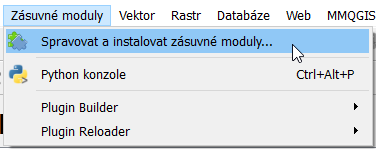
\includegraphics[width=.6\textwidth]{./pictures/otevreni_okna_zasuvne_moduly.png}
		\caption[Otevření okna \textit{Zásuvné
moduly}]{Otevření okna \textit{Zásuvné moduly}, zdroj: autor}
		\label{fig:manual_otevreni_okna_zasuvne_moduly}
 	\end{figure}
 	
V záložce \textit{Nastavení} zkontrolujte, zda je volba
\textit{Zobrazit také experimentální zásuvné moduly} aktivní.

Kliknutím na tlačítko \textit{Přidat...} připojíme repositář
laboratoře \textit{CTU GeoForAll
Lab}\footnote{\url{http://geomatics.fsv.cvut.cz/research/geoforall}}

\begin{lstlisting}[basicstyle=\footnotesize\ttfamily, backgroundcolor
= \color{light-gray}, numbers=left, columns=fullflexible,
keepspaces=true] Nazev: CVUT GeoForAll Lab URL:
http://geo.fsv.cvut.cz/geoforall/qgis-plugins.xml
\end{lstlisting}

	\begin{figure}[H] \centering
		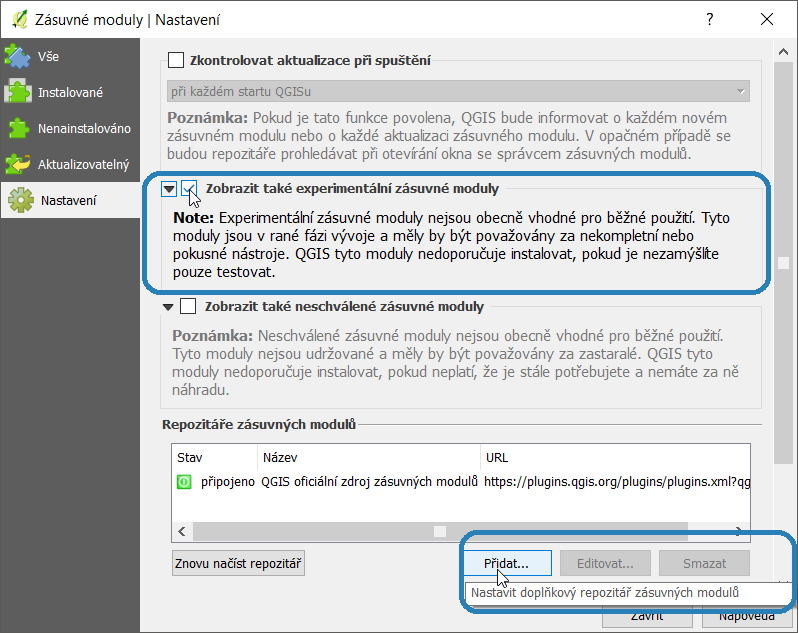
\includegraphics[width=.85\textwidth]{./pictures/pridani_repositare.png}
		\caption[Aktivování experimentálních zásuvných modulů
a přidání repositáře.]{Aktivování experimentálních zásuvných modulů a
přidání repositáře, zdroj: autor}
		\label{manual_pridani_repozitare}
 	\end{figure}
 	
	\begin{figure}[H] \centering
		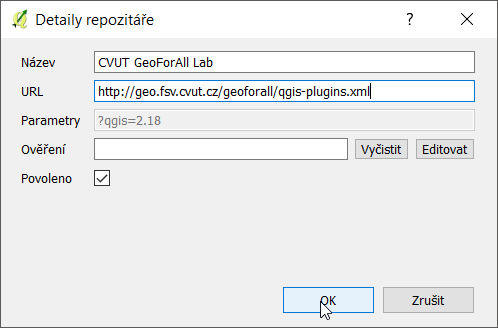
\includegraphics[width=.6\textwidth]{./pictures/zadani_repositare.png}
		\caption[Přidání repositáře GeoForAll Lab]{Přidání
repositáře CTU GeoForAll Lab, zdroj: autor}
		\label{manual_zadani_repozitare_geoforall_lab}
 	\end{figure}

\subsection{Instalace zásuvného modulu \textit{Soil Erosion}} Po
připojení repositáře vyhledejte \textit{Soil Erosion Plugin}, buďto v
záložce \textit{Vše} nebo \textit{Nenainstalované}. Po výběru
zásuvného modulu klikněte na \textit{Instalovat zásuvný modul}.

	\begin{figure}[H] \centering
		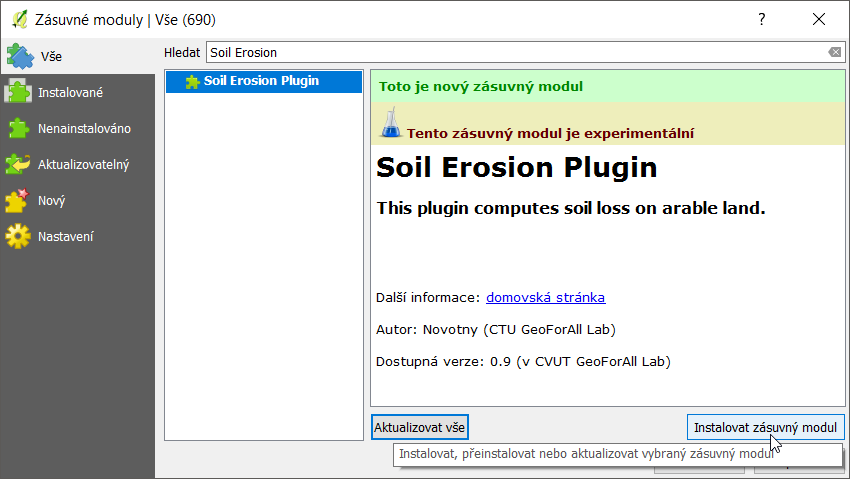
\includegraphics[width=.8\textwidth]{./pictures/instalace_pluginu.png}
		\caption[Instalace zásuvného modulu]{Instalace
zásuvného modulu, zdroj: autor}
		\label{fig:manual_pridani_repozitare_geoforall_lab}
 	\end{figure}
	
Po úspěšném nainstalování se v \textit{Panelu nástrojů Zásuvné moduly}
objeví jeho ikona. Zásuvný modul je možné spustit kliknutím na jeho
ikonu nebo z menu \textit{Zásuvné moduly} $\rightarrow$ \textit{Soil
Erosion} $\rightarrow$ \textit{Soil Erosion Plugin}.
	
	\begin{figure}[H] \centering
		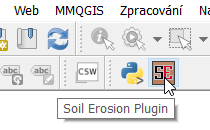
\includegraphics[width=.3\textwidth]{./pictures/spusteni_pluginu2.png}
		\caption[Ikona zásuvného modulu v panelu
nástrojů]{Ikona zásuvného modulu v panelu nástrojů, zdroj: autor}
		\label{ikona_modulu_v_panelu_nastroju}
 	\end{figure}
	
	\begin{figure}[H] \centering
		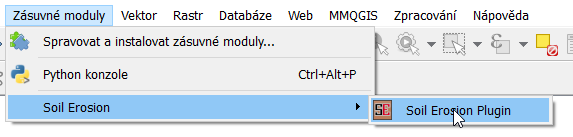
\includegraphics[width=.7\textwidth]{./pictures/spusteni_pluginu1.png}
		\caption[Ikona zásuvného modulu v menu]{Ikona
zásuvného modulu v menu, zdroj: autor}
		\label{ikona_modulu_v_panelu_nastroju2}
 	\end{figure}

\section{Návod k použití}
\label{navod_k_pouziti} Pro vytvoření erozního modelu je nutné
vyplnění pěti záložek, ve kterých jsou definovány pozemky, na kterých
bude výpočet probíhat (EUC), a voleny vstupy pro určení faktorů v
rovnici USLE (LS, K, C a RP).
\subsection{EUC} Určení erozně uzavřených celků (pozemků), pro které
bude určována průměrná roční ztráta, probíhá v záložce EUC.

	\begin{figure}[H] \centering
		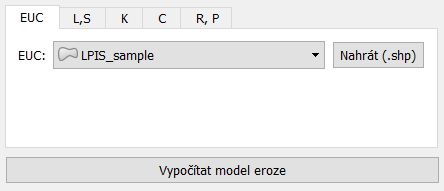
\includegraphics[width=.5\textwidth]{./pictures/euc.png}
		\caption[Záložka EUC]{Záložka EUC, zdroj: autor}
		\label{zalozka_euc}
 	\end{figure}

Zde se volí polygonová vektorová vrstva (.shp) definující EUC. Vrstvu
je možné zvolit ze seznamu vrstev, či ji nahrát přes tlačítko
\textit{Nahrát (.shp)}.

Tato vrstva většinou vychází z vrstvy LPIS, ovšem je rovněž možné
volit svou vlastní vrstvu. Ovšem při zvolení vlastní vrstvy je potřeba
dát pozor, aby na většině plochy EUC byly definovány faktory K a C.

\paragraph{Poznámka:} Při využítí vrstvy LPIS je pro správnou
funkčnost výpočtu doporučeno zkontrolovat návaznosti polygonů. Zda v
místech, kde se jedná o jeden EUC rozdělený mezi několik vlastníků
(uživatelů), na sebe polygony navazují (případně se překrývají). (EUC
1A a EUC 1B)

Naopak v místech, kde jsou pozemky erozně odděleny technické
protierozním opatření či silnicí, musí být mezi jednotlivými polygony
mezera. (EUC 2 a EUC 3)
\begin{figure}[H] \centering
		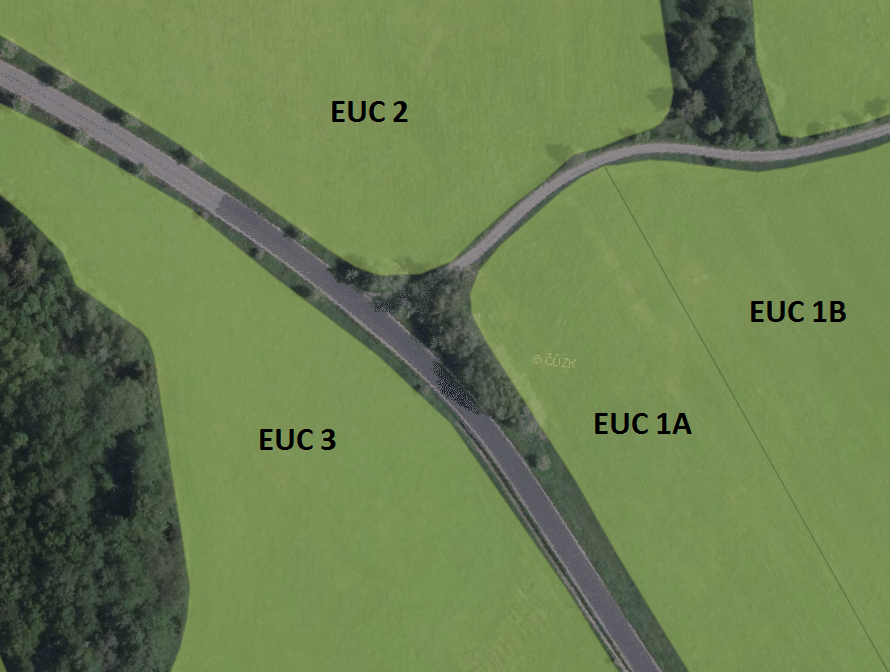
\includegraphics[width=.7\textwidth]{./pictures/rozdeleni_euc.png}
		\caption[Zobrazení EUC se zahrnutými
překážkami]{Zobrazení EUC se zahrnutými překážkami, zdroj: autor}
		\label{rozdeleni_euc}
\end{figure} Pro základní kontrolu je vhodné využití ortofota.
\subsection{L,S} V záložce L,S se určuje rastr digitálního modelu
terénu, nad kterým bude probíhat výpočet faktorů délky a sklonu svahu
(L, S). Vrstvu je možné zvolit ze seznamu vrstev, či ji nahrát přes
tlačítko \textit{Nahrát (rastr)}.
\begin{figure}[H] \centering
		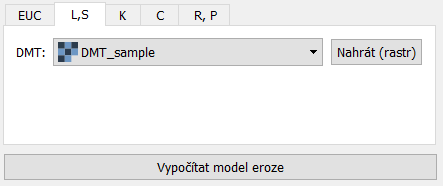
\includegraphics[width=.6\textwidth]{./pictures/ls.png}
		\caption[Záložka L,S]{Záložka L,S, zdroj: autor}
		\label{zalozka_ls}
\end{figure}
\subsection{K} V záložce K se volí polygonová vektorová vrstva (.shp)
BPEJ. Vrstva musí obsahovat pole s názvem \uv{BPEJ} ve formátu
\uv{X.XX.XX}, ze kterého se pomocí tlačítka \textit{Vypočítat K
faktor}, vypočte hodnota K a vrstva se dle jeho hodnoty barevně
rozliší. Případně je možné použít vrstvu s předem vypočteným K
faktorem v poli \textit{K}. Vrstvu je možné zvolit ze seznamu vrstev,
či ji nahrát přes tlačítko \textit{Nahrát (.shp)}.
\begin{figure}[H] \centering
		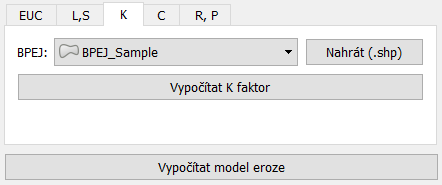
\includegraphics[width=.6\textwidth]{./pictures/k.png}
		\caption[Záložka K]{Záložka K, zdroj: autor}
		\label{zalozka_k}
\end{figure}
\paragraph{Tip:} Hodnoty K lze poté manuálně upravovat v atributové
tabulce (stejně lze upravovat i hodnoty C)
\subsection{C} Záložka C slouží ke zvolení polygonové vektorové vrstvy
(.shp) LPIS. Vrstva musí obsahovat pole s názvem \uv{KULTURAKOD} s
jednoznakovým kódem pro využití pozemku. V rolovací nabídce se volí
primární osevní postup užívaný na pozemcích s ornou půdou. Poté se C
faktor nastaví kliknutím na tlačítko \textit{Vypočítat C faktor},
přičemž současně dojde k barevnému rozlišení dle využití pozemku.
\begin{figure}[H] \centering
		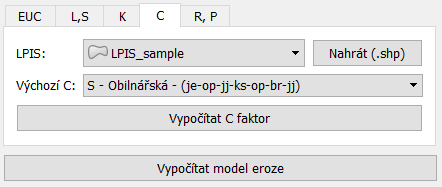
\includegraphics[width=.6\textwidth]{./pictures/c.png}
		\caption[Záložka C]{Záložka C, zdroj: autor}
		\label{zalozka_c}
\end{figure}
\paragraph{Poznámka:} Při využití dat LPIS vyexportovaných z Registru
půd
(LPIS)\footnote{\url{http://eagri.cz/public/app/eagriapp/lpisdata/}}
a~BPEJ\footnote{\url{http://www.spucr.cz/bpej/celostatni-databaze-bpej}}
z celostátní databáze, jejich formát odpovídá požadavkům zásuvného
modulu.
\paragraph{Tip:} Hodnoty C lze poté manuálně upravovat v atributové
tabulce (stejně lze upravovat i hodnoty K)
\subsection{R,P} V poslední záložce \textit{R,P} je možné upravit
hodnotu faktoru přívalového deště \textit{R} pro danou oblast. Tato
hodnota je nastavena na 40, což je průměrná hodnota pro ČR. Dále pak
hodnotu faktoru protierozních opatření \textit{P}, ta je nastavena na
1 (= Nejsou použita žádná agrotechnická protierozní opatření.)
\begin{figure}[H] \centering
		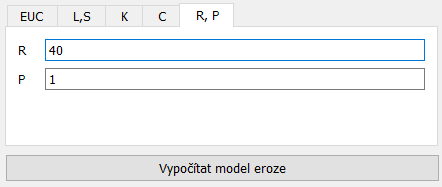
\includegraphics[width=.55\textwidth]{./pictures/rp.png}
		\caption[Záložka RP]{Záložka RP, zdroj: autor}
		\label{zalozka_rp}
\end{figure}
\subsection{Výpočet erozního modelu} Po nastavení všech vstupních
hodnot se stisknutím tlačítka provede výpočet erozního
modelu. Tlačítko je viditelné ze všech záložek. Po spuštění výpočtu
jsou zobrazovány informace o jeho průběhu pomocí panelu v horní části
QGIS. Z tohoto panelu je také možné výpočet ukončit pomocí tlačítka
\textit{Zrušit výpočet}.
\begin{figure}[H] \centering
		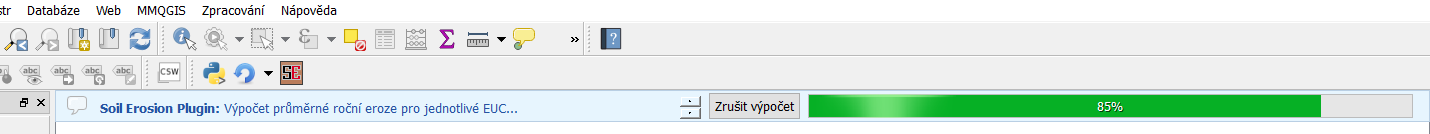
\includegraphics[width=.9\textwidth]{./pictures/progressbar.png}
		\caption[Informačního panel]{Informační panel,
zdroj: autor}
		\label{informacni_panel}
\end{figure}
\subsection{Erozní model} Po skončení výpočtu se do mapového okna na
první a druhé místo v seznamu vrstev přidají vrstvy erozního modelu -
\textit{EUC} a \textit{Lokální eroze}. Ukázku těchto vrstev je možné
najít v popisu ukázkového výpočtu.
\begin{itemize}
	\item Erozní model: Vektorová polygonová vrstva \textit{EUC}
je vytvořená z vrstvy zadané v záložce EUC. Do atributové tabulky této
vrstvy je přidán nový sloupec G s hodnotou průměrné roční ztráty půdy
pro jednotlivé pozemky, tyto pozemky jsou rovněž obarveny dle tabulky
ohrožení půdy.
	\item G faktor: Rastrová vrstva zobrazující lokální hodnoty
eroze ve stupních šedi.
\end{itemize} Při spuštění nového výpočtu se vytvořené vrstvy nahradí
novými.

\section{Ukázkový výpočet}

\subsection{Vzorová data} Pro ukázkový výpočet jsou použita vzorová
data. Ta obsahují 3 vrstvy \textit{DMT\_sample}, \textit{BPEJ\_Sample}
a \textit{LPIS\_Sample}.
%%% ML: chybi odkaz na testovaci data umistena v Git repozitari
\begin{figure}[H] \centering
		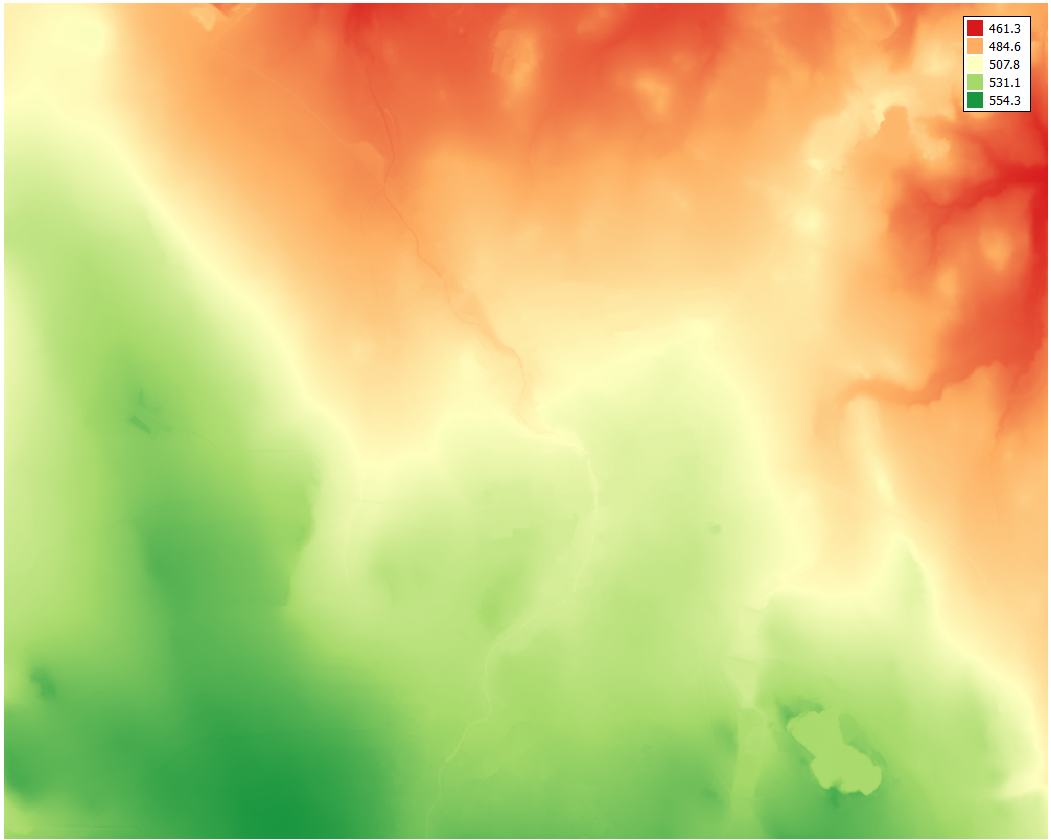
\includegraphics[width=.4\textwidth]{./pictures/dmt_layer1.png}
		\caption[Vrstva DMT\_sample]{Vrstva DMT\_sample,
zdroj: autor}
		\label{dmt_sample}
\end{figure}
\begin{figure}[H] \centering
		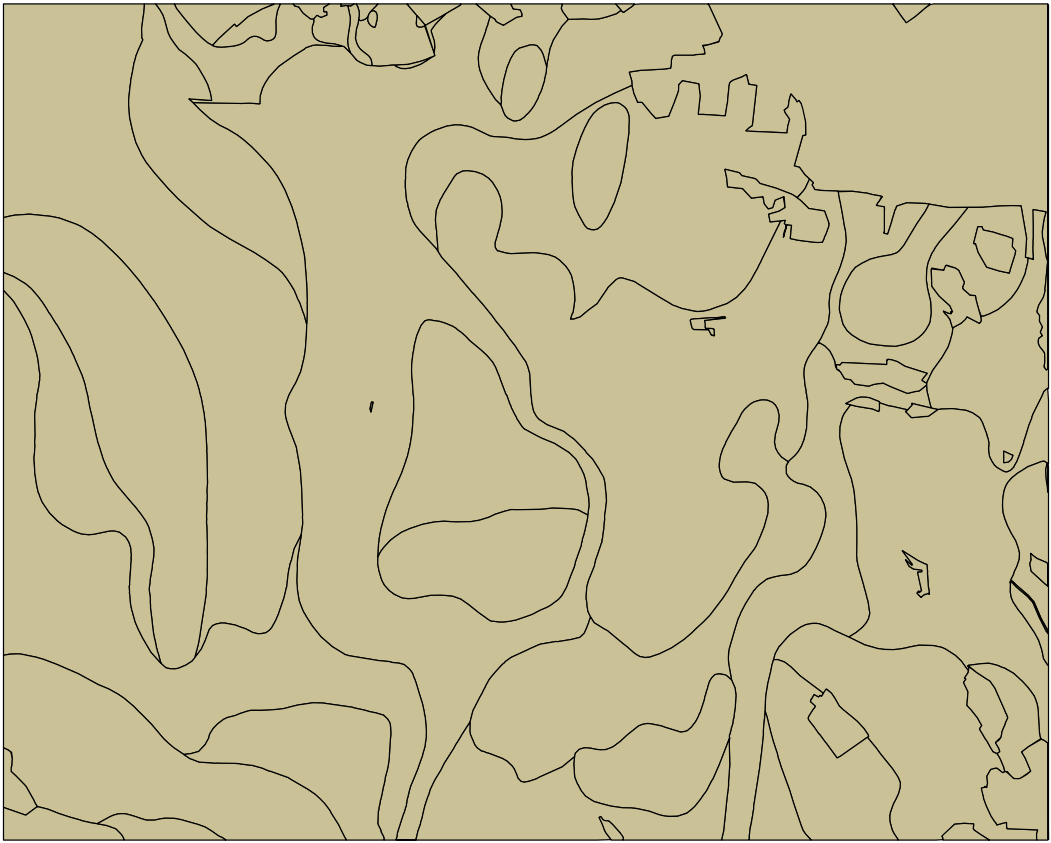
\includegraphics[width=.4\textwidth]{./pictures/bpej_layer1.png}
		\caption[Vrstva BPEJ\_sample]{Vrstva BPEJ\_sample,
zdroj: autor}
		\label{bpej_sample}
\end{figure}
\begin{figure}[H] \centering
		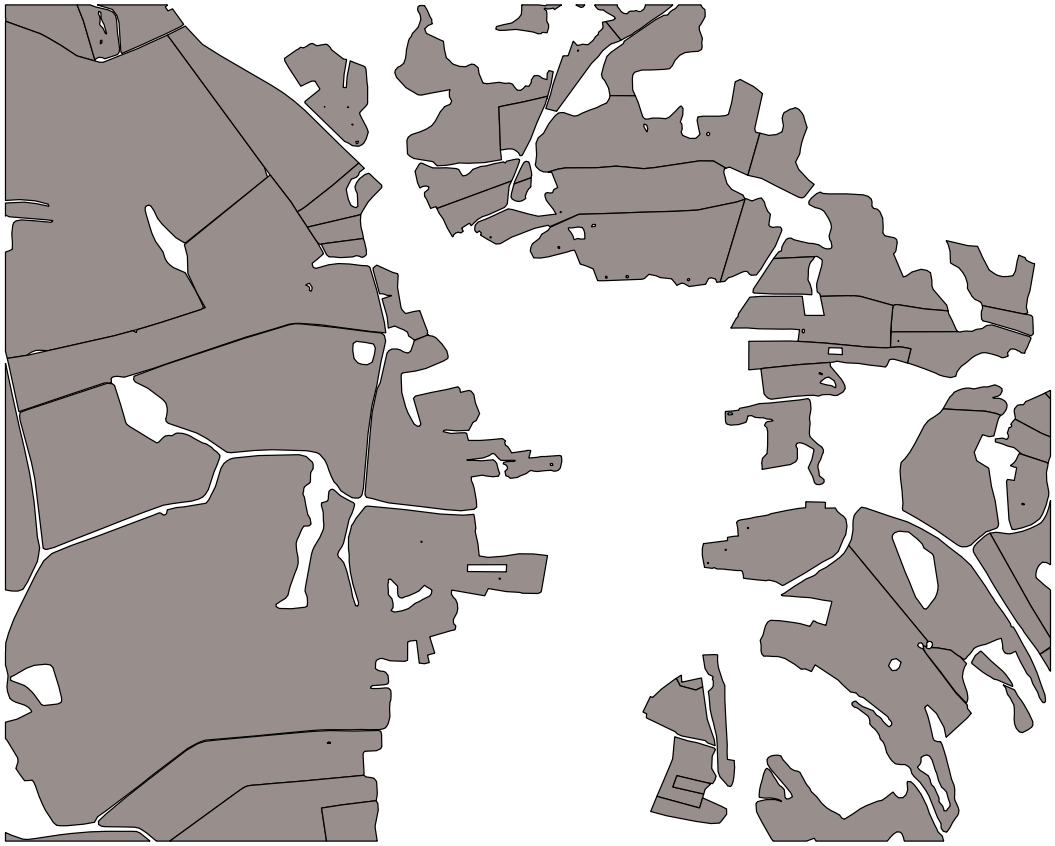
\includegraphics[width=.4\textwidth]{./pictures/lpis_layer1.png}
		\caption[Vrstva LPIS\_sample]{Vrstva LPIS\_sample,
zdroj: autor}
		\label{lpis_sample}
\end{figure}
\subsection{Nastavení vstupů a výpočet} Nastavení vstupních hodnot se
provede podle obecného návodu, kdy se jako EUC vrstva zvolí
%%% ML: nebavili jsme se o tom, ze se vrtsva EUC bude mirne od LPIS
%%% lisit? (tak jak to mate popsano v textu)
LPIS\_sample, v následujících záložkách názvy požadovaných vrstev
odpovídají jménu vzorových dat. Po výpočtu faktorů K a C v daných
záložkách se vrstvy obarví.
\begin{figure}[H] \centering
		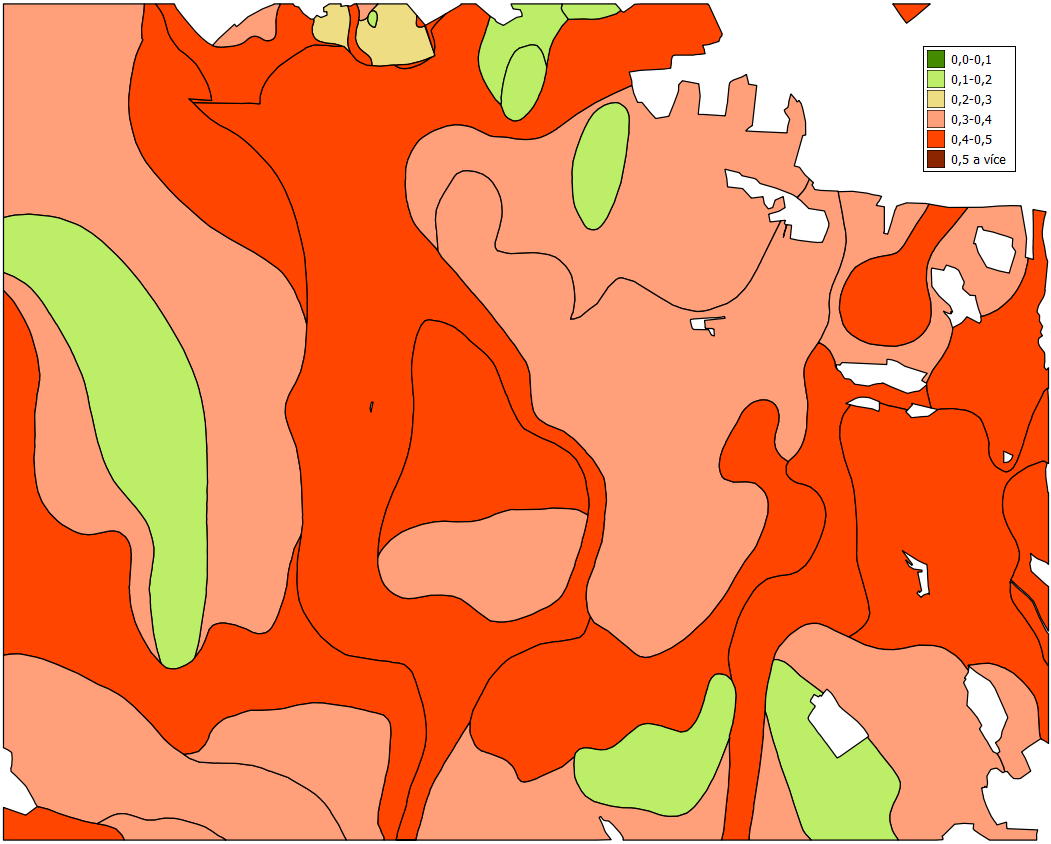
\includegraphics[width=.5\textwidth]{./pictures/bpej_layer2.png}
		\caption[Vrstva BPEJ\_sample po výpočtu K
faktoru]{Vrstva BPEJ\_sample po výpočtu K faktoru, zdroj: autor}
		\label{bpej_sample2}
\end{figure}
\begin{figure}[H] \centering
		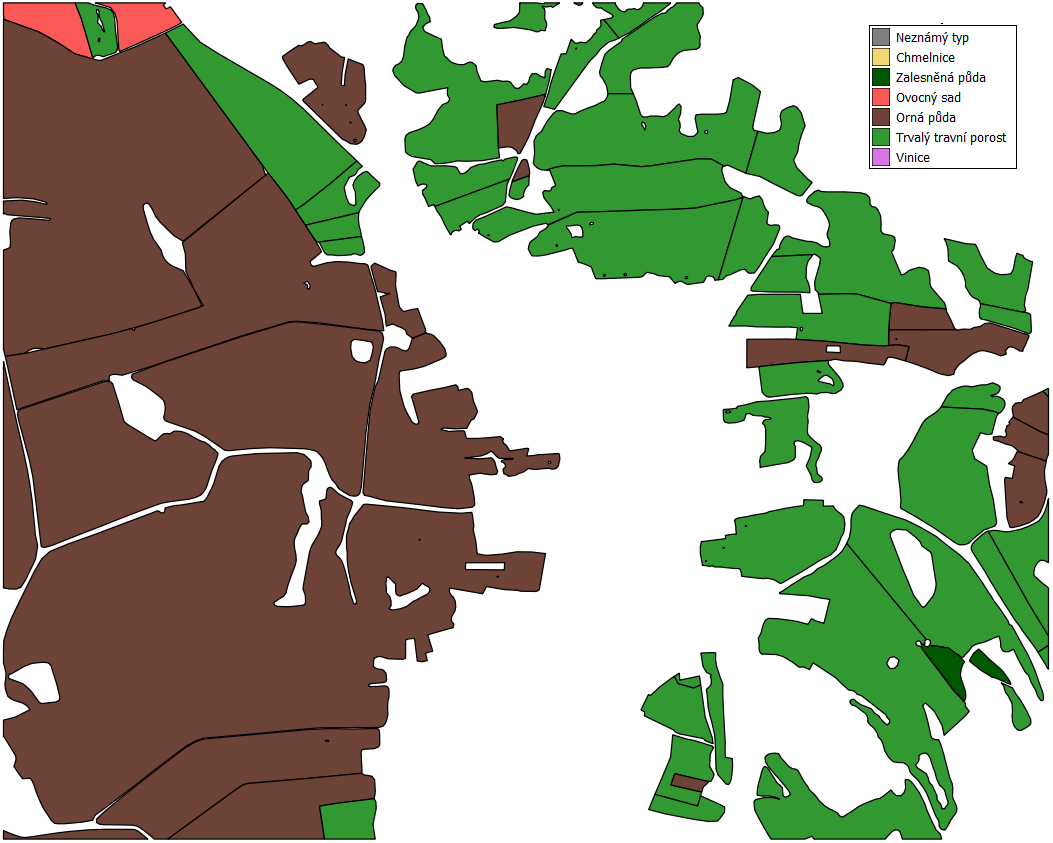
\includegraphics[width=.5\textwidth]{./pictures/lpis_layer2.png}
		\caption[Vrstva LPIS po výpočtu C faktoru]{Vrstva LPIS
po výpočtu C faktoru, zdroj: autor}
		\label{lpis_sample2}
\end{figure} V poslední záložce R,P jsou ponechány výchozí hodnoty a
plugin je spuštěn.
\newpage
\subsection{Výsledný model} Výsledkem výpočtu by měly být následující
vrstvy:
\begin{figure}[H] \centering
		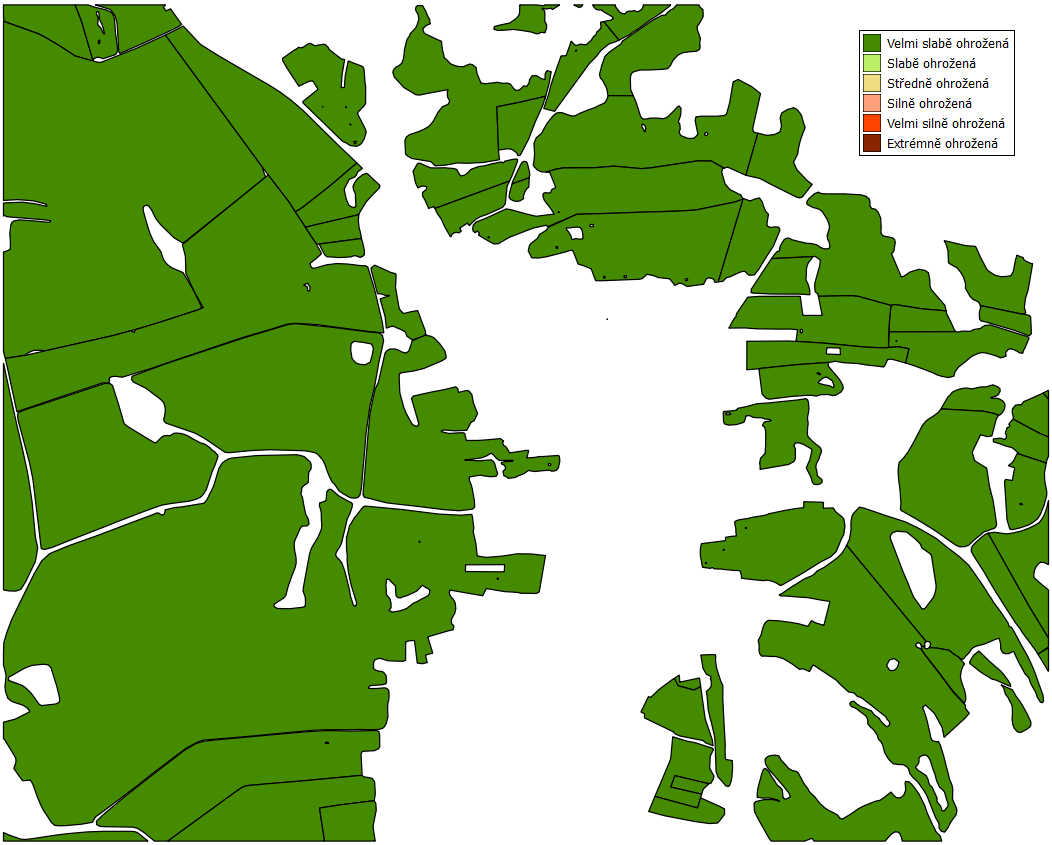
\includegraphics[width=.5\textwidth]{./pictures/euc_layer.png}
		\caption[Vrstva EUC]{Vrstva EUC, zdroj: autor}
		\label{euc_sample}
\end{figure}
\paragraph{Poznámka:} Výsledná vrstva EUC je jednolitá z důvodu nízké
erozní ohroženosti oblasti. Tato oblast ovšem musela být vybrána z
důvodu využití vzorových (volně šiřitelných) dat DMT z DMR 5G.
\begin{figure}[H] \centering
		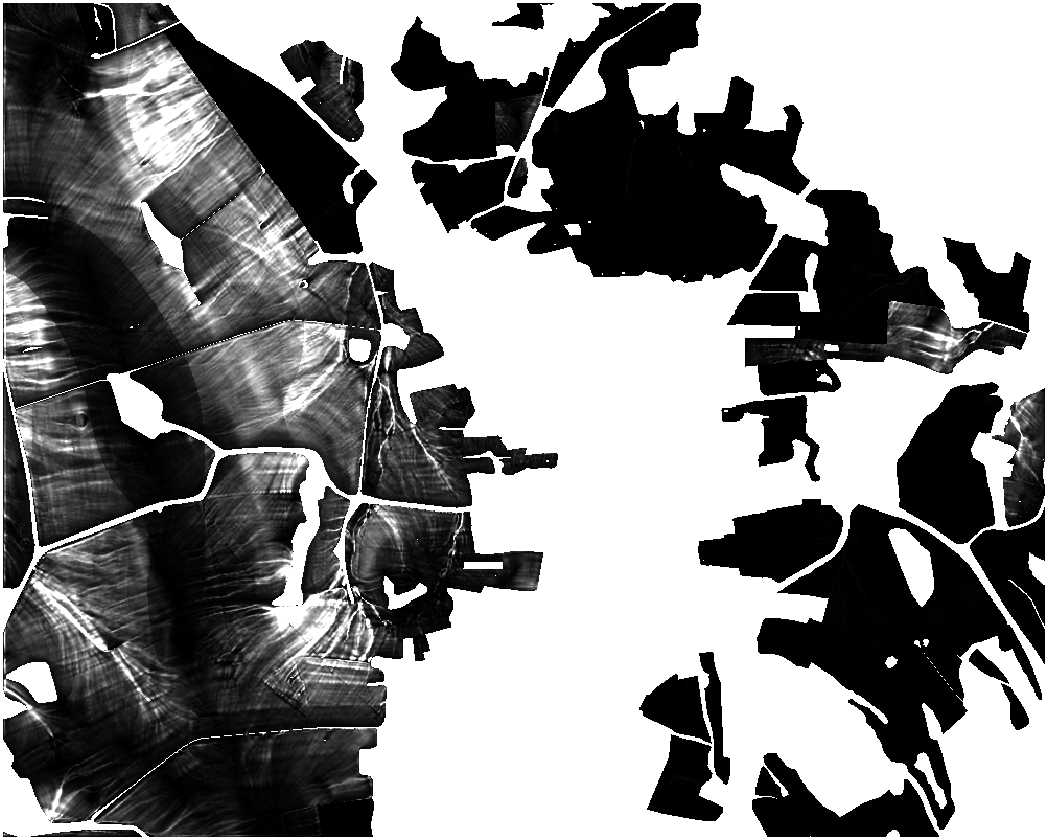
\includegraphics[width=.5\textwidth]{./pictures/lokalni_eroze_layer.png}
		\caption[Vrstva G faktor]{Vrstva G faktor, zdroj:
autor}
		\label{g_sample}
              \end{figure}
              
%%% ML: text nize bych v priloze neuvadel
              
% \section{Autoři} Pro Labolatoř GeoForAll - České vysoké učení
% technické v Praze

% Jako bakalářskou práci vytvořil Radek Novotný pod vedením Ing. Martina
% Landy, PhD.